%%%%%%%%%%%%%%%%%%%%%%%
% ADDITIONAL NUISANCE %
%%%%%%%%%%%%%%%%%%%%%%%
In the following we describe an experimental situation where the inference of the QoI \(\bm{\theta}_E\) is hampered by additional uncertainties in the experimental conditions.
Experimental conditions are formally treated as nuisance parameters with prescribed uncertainties.
More specifically, we do not assume that the loads \(F_i\) are perfectly known anymore.
In contrast, we assume that they are \(\bm{\zeta}_i\)-type variables, i.e.\ they are uncertain yet they follow a known distribution.
% EXPERIMENTAL SITUATION
This represents a well-known situation where the loads \(F_i\) that the testing machine actually applies can only be imprecisely adjusted.
In fact, while a targeted load in each experiment is chosen, the physically realized load \(F_i\) may be uncertain.
This is accounted for by a prescribed distribution \(\mathcal{N}(F_i \distparam \mu_{F_i},\sigma_{F_i}^2)\)
where \(\mu_{F_i}\) is the targeted load and \(\sigma_{F_i}\) represents the degree of uncertainty that is inherent to the test machinery.
\par % NUMERICAL SETUP
The setup for conducting a numerical experiment is similar to the one specified in \cref{sec:PEM:CaseStudies:ProbInv}.
For \(n=50\) beams we set the beam dimensions \(\bm{l}_i\) and measurement positions \(\bm{s}_i\) as before.
Elastic moduli \(E_i\) are randomly drawn from \(\mathcal{LN}(E_i \cond \mu_E,\sigma_E)\) as previously detailed.
In contrast to plain probabilistic inversion, for \(i=1,\ldots,n\) experiment-specific loads \(F_i\) are independently sampled from
normal distributions \(\mathcal{N}(F_i \distparam \mu_{F_i},\sigma_{F_i}^2)\) with \(\mu_{F_i} = \unit[30]{kN}\) and \(\sigma_{F_i} = \unit[3]{kN}\).
This equates to a coefficient of variation \(c_{F_i} = \unit[10]{\%}\).
% COMMENTS
Note that such a high degree of uncertainty is unlikely to be encountered in a real-case experiment.
It is used here to accentuate the results presented below, though.
% TREATED AS UNKNOWNS
The realized loads \(F_i\) will be treated as unknowns whereas the hyperparameters \(\bm{\theta}_{F_i} = (\mu_{F_i},\sigma_{F_i})\), i.e.\ the targeted load and its uncertainty, will be treated as knowns.
% PSEUDO MEASUREMENTS
In accordance with \cref{eq:PEM:Beams:AlgebraicFormula} synthetic measurements \(\bm{v}_i = \perfect{\bm{v}}_i + \bm{\varepsilon}_i\) are generated again.
% HYPERPRIORS
The prior distribution \(\pi(\bm{\theta}_E) = \pi(\mu_E) \, \pi(\sigma_E)\) is also chosen as previously stated.
\par % SUMMARY
The problem of probabilistic inversion under additional prescribed nuisance reads as follows.
The hyperparameters \(\bm{\theta}_{\bm{X}} \equiv \bm{\theta}_E\) are the QoI
whereas experiment-specific unknowns \(\tuple{\bm{x}_i} \equiv \tuple{E_i}\) and \(\tuple{\bm{\zeta}_i} \equiv \tuple{F_i}\) are considered nuisance.
With measurements \(\tuple{\bm{y}_i} \equiv \tuple{\bm{v}_i}\) the QoI can be inferred.
Experimental-specific knowns consist of the hyperparameters \(\tuple{\bm{\theta}_{\bm{Z}_i}} \equiv \tuple{\bm{\theta}_{F_i}}\),
the experimental conditions \(\tuple{\bm{d}_i} \equiv \tuple{(\bm{l}_i,\bm{s}_i)}\) and the residual covariances \(\tuple{\bm{\Sigma}_i}\).
Parametric Bayesian prior knowledge is given by \(\pi_{\bm{\Theta}_{\bm{X}}}(\bm{\theta}_{\bm{X}}) \equiv \pi(\bm{\theta}_E)\)
whereas \(f_{\bm{X} \cond \bm{\Theta}_{\bm{X}}} (\bm{x}_i \cond \bm{\theta}_{\bm{X}}) \equiv \mathcal{LN}(E_i \cond \mu_E,\sigma_E)\) and 
\(f_{\bm{Z}}(\bm{\zeta}_i \distparam \bm{\theta}_{\bm{Z}_i}) \equiv \mathcal{N}(F_i \distparam \mu_{F_i},\sigma_{F_i}^2)\) are structural prior distributions.
Within a joint approach a posterior of the form \(\pi( \tuple{\bm{x}_i},\tuple{\bm{\zeta}_i},\bm{\theta}_{\bm{X}} \cond \tuple{\bm{y}_i}) \equiv \pi( \tuple{E_i},\tuple{F_i},\bm{\theta}_E \cond \tuple{\bm{v}_i})\) arises.
Eventually one is interested in the QoI-marginals \( \pi(\bm{\theta}_{\bm{X}} \cond \tuple{\bm{y}_i}) \equiv \pi(\bm{\theta}_E \cond \tuple{\bm{v}_i})\) only.
% DAG
A DAG corresponding to this experimental situation is shown in \cref{fig:PEM:DAG:AddPres}.

\subsubsection{Results: Hyperparameters}
% PROBLEM FORMULATIONS
We sample the joint posterior \(\pi(\tuple{E_i},\tuple{F_i},\bm{\theta}_E \cond \tuple{\bm{v}_i})\) where nuisance variables \(\tuple{F_i}\) are explicitly accounted for.
% BLOCKSWISE MCMC
In a blockwise manner MCMC sweeps are accomplished for \((\mu_E,\sigma_E)\), \(\tuple{E_i}\) and \(\tuple{F_i}\) which constitute different blocks.
Blockwise proposal distributions are again adjusted in order to obtain acceptance rates in between \(\unit[20]{\%}\) and \(\unit[40]{\%}\).
% INITIALIZATION
Each \(F_i\) in the block \(\tuple{F_i}\) is initialized at \(F_i^{(0)} = \mu_{F_i}\), i.e.\ the structural prior mean.
% CONVERGENCE CHECKS
Other than that initialization, convergence checks and burn-in are accomplished as before.
% COMPUTATION TIME
For \(N=10^7\) MCMC iterations the total computation time amounts to \(t=\unit[7.18]{h}\).
% POSTERIOR MARGINALS
The resulting posterior marginals of \(\mu_E\) and \(\sigma_E\) can be seen in \cref{fig:PEM:AddPres:Marginals}.
A statistical summary is provided in \cref{tab:PEM:AddPres:Summary} where the mean, mode, SD and CV of the marginals are itemized.
% MARGINAL POSTERIORS
\begin{figure}[ht]
  \centering
  \begin{subfigure}[b]{0.5\textwidth}
    \centering
    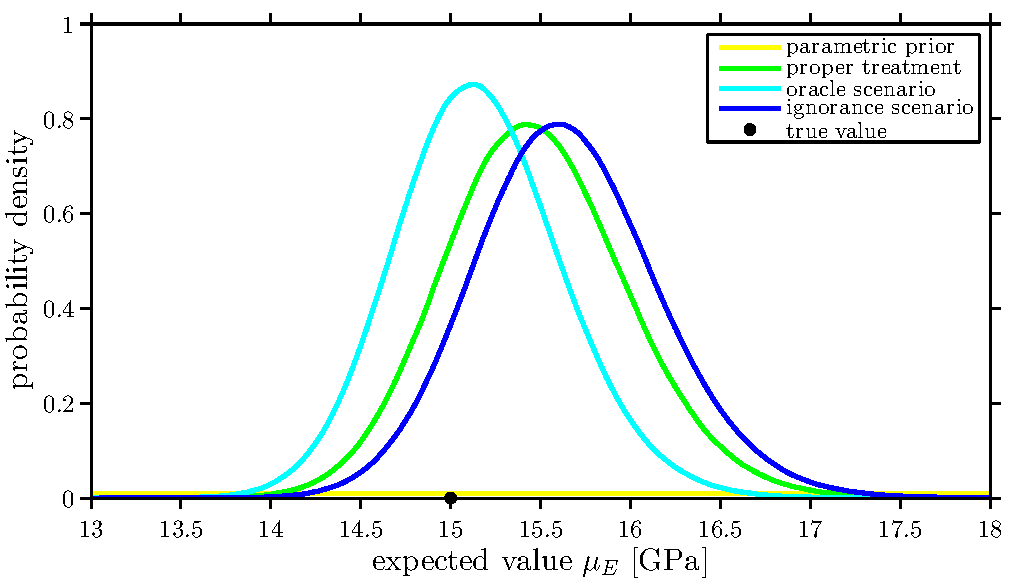
\includegraphics[height=\PEMfigHeight]{fig_PEM_AddPresPostMean}
    \caption{Posterior marginal of \(\mu_E\).}
    \label{fig:PEM:AddPres:Post:Mean}
  \end{subfigure}%
  \begin{subfigure}[b]{0.5\textwidth}
    \centering
    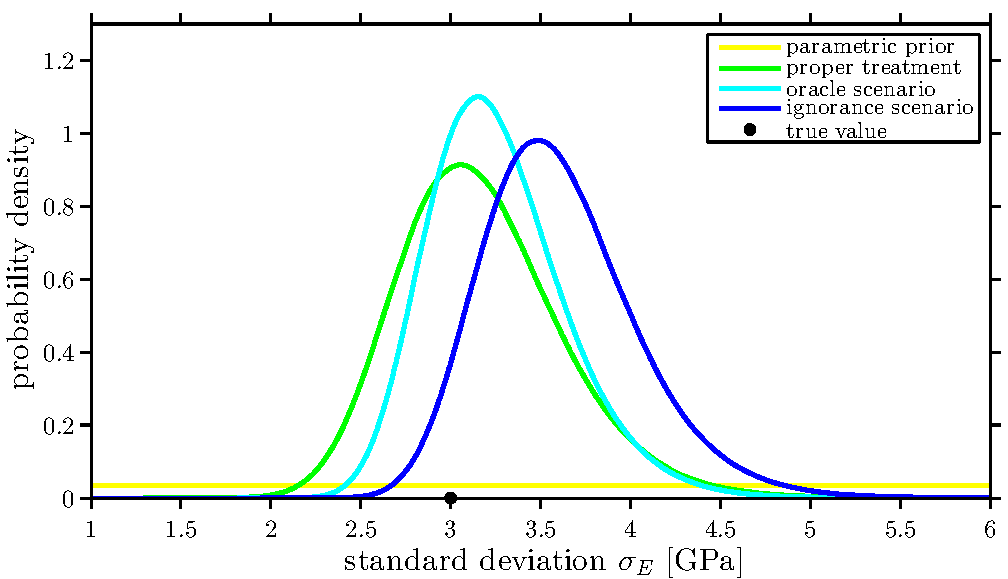
\includegraphics[height=\PEMfigHeight]{fig_PEM_AddPresPostSigma}
    \caption{Posterior marginal of \(\sigma_E\).}
    \label{fig:PEM:AddPres:Post:Sigma}
  \end{subfigure}%
  \caption[Posterior marginals of the QoI]{Posterior marginals of the QoI.
           The marginal posteriors of \(\mu_E\) and \(\sigma_E\) are provided in \subref{fig:PEM:AddPres:Post:Mean} and \subref{fig:PEM:AddPres:Post:Sigma}, respectively.
           Three experimental scenarios are investigated: the proper treatment of the additional uncertainty, 
           an idealized situation where one would precisely know the loads, and the case of a parsimonious model where the uncertainty remains unrecognized.
          }
  \label{fig:PEM:AddPres:Marginals}
\end{figure}
% TABLE: ADDITIONAL PRESCRIPTION
\begin{table}[ht]
  \caption[Summary of the QoI posterior marginals]{Summary of the QoI posterior marginals.}
  \label{tab:PEM:AddPres:Summary}
  \centering
  \begin{tabular}{lcccccccccc}
    \toprule
      & \phantom{} & \multicolumn{3}{c}{\(\mu_E\) \(\lbrack\unit[]{GPa}\rbrack\)} & \(\lbrack \unitless \rbrack\)
      & \phantom{} & \multicolumn{3}{c}{\(\sigma_E\) \(\lbrack\unit[]{GPa}\rbrack\)} & \(\lbrack \unitless \rbrack\) \\
    \cmidrule{3-6} \cmidrule{8-11}
    && Mean & Mode & SD & CV && Mean & Mode & SD & CV \\
    \midrule
    Proper treatment   && \(15.47\) & \(15.41\) & \(0.51\) & \(0.03\) && \(3.17\) & \(3.05\) & \(0.46\) & \(0.14\) \\
    Oracle scenario    && \(15.16\) & \(15.13\) & \(0.47\) & \(0.03\) && \(3.26\) & \(3.15\) & \(0.39\) & \(0.12\) \\
    Ignorance scenario && \(15.65\) & \(15.60\) & \(0.52\) & \(0.03\) && \(3.61\) & \(3.51\) & \(0.43\) & \(0.12\) \\
    \bottomrule
  \end{tabular}
\end{table}
\par % POSTERIOR SIGNIFICANCE
We try to assess the impact of the uncertainty that had been introduced in the loads \(F_i\) on the estimation of the QoI \(\bm{\theta}_E = (\mu_E,\sigma_E)\).
To that end we pursue the following two strategies.
% IDEALIZED SITUATION
First of all we estimate the QoI while treating the realized loads \(F_i\) as if they were part of the experiment-specific knowns \(\bm{d}_i\).
This ``what-if'' or ``oracle'' scenario actually describes the hypothetical situation that we met in plain probabilistic inversion.
It does not describe the realistic scenario of uncertain conditions \(\bm{\zeta}_i\) that we are actually investigating.
Yet this way of proceeding sheds light on how the prescribed uncertainty in the loads affects the inference of the QoI.
% INTERPRETATION
For \(N=10^7\) and \(t=\unit[4.33]{h}\) the results to probabilistic inversion are added to \cref{fig:PEM:AddPres:Marginals}.
With respect to this idealized situation, one can reassess the previous results of properly treating the loads as uncertain.
The introduction of the uncertainty in the loads had actually shifted the posterior modes and raised the level of estimation uncertainty accordingly.
\par % UNCERECOGNIZED UNCERTAINTY
Second of all we investigate the case that the uncertainty \(\mathcal{N}(F_i \distparam \mu_{F_i},\sigma_{F_i}^2)\) in the applied loads \(F_i\) is simply disregarded.
Either it has not been recognized by mistake or it has been intentionally dropped by making simplifying assumptions in favor of a parsimonious model.
% MISTREATMENT
Rather than treating the loads as belonging to the unknowns \(\bm{\zeta}_i\), we erroneously treat them as such experimental conditions \(\erroneous{\bm{d}}_i\) that only approximately describe the prevailing conditions \(\bm{d}_i\).
While the data has been created under \(\bm{d}_i\), data analysis is carried out under \(\erroneous{\bm{d}}_i\).
% EXPERIMENTAL SITUATION
This describes a situation where the experimenter targets a load \(\erroneous{F}_i = \mu_{F_i}\), but the testing machine actually realizes \(F_i\).
If this uncertainty \(\mathcal{N}(F_i \distparam \mu_{F_i},\sigma_{F_i}^2)\) is not accounted for or not recognized at all,
the analyst will accomplish inference under the spurious assumption that the loads had taken on their targeted values \(\erroneous{F}_i\) during experiment execution.
% RESULTS & INTERPRETATION
For \(N=10^7\) and \(t=\unit[3.75]{h}\) the resulting posteriors are added to \cref{fig:PEM:AddPres:Marginals}.
Our interpretation is that dropping the uncertainty of \(F_i\) corrupts the estimation of the QoI and results in misleading estimates of posterior uncertainty,
whereas the proper treatment of all uncertainties yields results that are closer to the idealized ``oracle'' scenario.

\subsubsection{Results: Intermediate variables}
\par % FURTHER INSIGHTS
Sampling the joint posterior \(\pi(\tuple{E_i},\tuple{F_i},\bm{\theta}_E \cond \tuple{\bm{v}_i})\) of the entirety of unknowns provides further interesting insights.
% POSTERIOR OF THE LOADS
Apart from the QoI-marginals one can examine the posterior model of experiment-specific loads \(F_i\), notwithstanding that they are considered nuisance.
\cref{fig:PEM:AddPres:Posteriors} contains two different posteriors involving some \(F_i\).
In \cref{fig:PEM:AddPres:Post:1DLoad} the posterior marginal of a pinpoint load \(F_i\) is shown for \(i=23\).
The identification of specifically applied loads \(F_i\) is subject to rather high levels of posterior uncertainty.
% IDENTIFIABILITY
This is an issue of statistical identifiability.
When both \(E_i\) and \(F_i\) are uncertain and various combinations of these can explain the observation \(\bm{v}_i\) equally well, then those combinations \((E_i,F_i)\) cannot be distinguished a posteriori.
Of course, the reason is that only the ratio \(F_i/E_i\) in \cref{eq:PEM:Beams:AlgebraicFormula} can be identified.
% POSTERIOR CORRELATION
It is therefore interesting to investigate the posterior correlation between the load \(F_i\) and the modulus \(E_i\) of an experiment \(i\).
The two-dimensional posterior of \((E_i,F_i)\) for \(i=20\) that is shown in \cref{fig:PEM:AddPres:Post:2DMeanLoad} serves as an example.
Posterior mass is assigned to suitable parameter constellations \((E_i,F_i)\) that well-explain the measurement \(\bm{v}_i\).
As expected the posterior is strongly correlated with a linear coefficient of correlation \(r_{F_{20},E_{20}} = 0.99\).
% POSTERIORS: ADDITIONAL PRESCRIPTION
\begin{figure}[ht]
  \centering
  % MARGINAL POSTERIOR: APPLIED LOAD
  \begin{subfigure}[b]{0.5\textwidth}
    \centering
    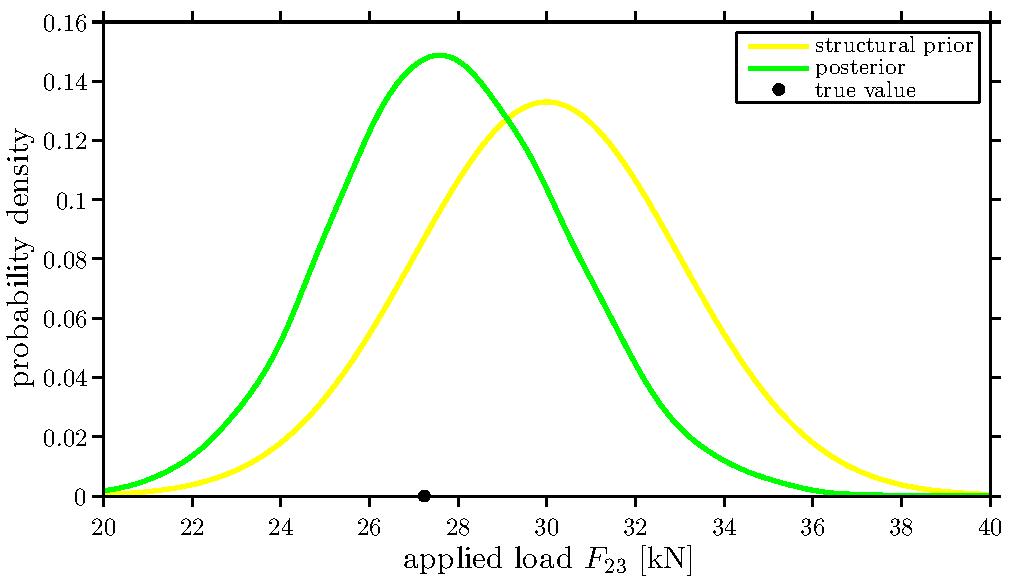
\includegraphics[height=\PEMfigHeight]{fig_PEM_AddPresPostLoad}
    \caption{Posterior marginal of \(F_{23}\).}
    \label{fig:PEM:AddPres:Post:1DLoad}
  \end{subfigure}%
  % 2D POSTERIOR: LOAD-MODULUS
  \begin{subfigure}[b]{0.5\textwidth}
    \centering
    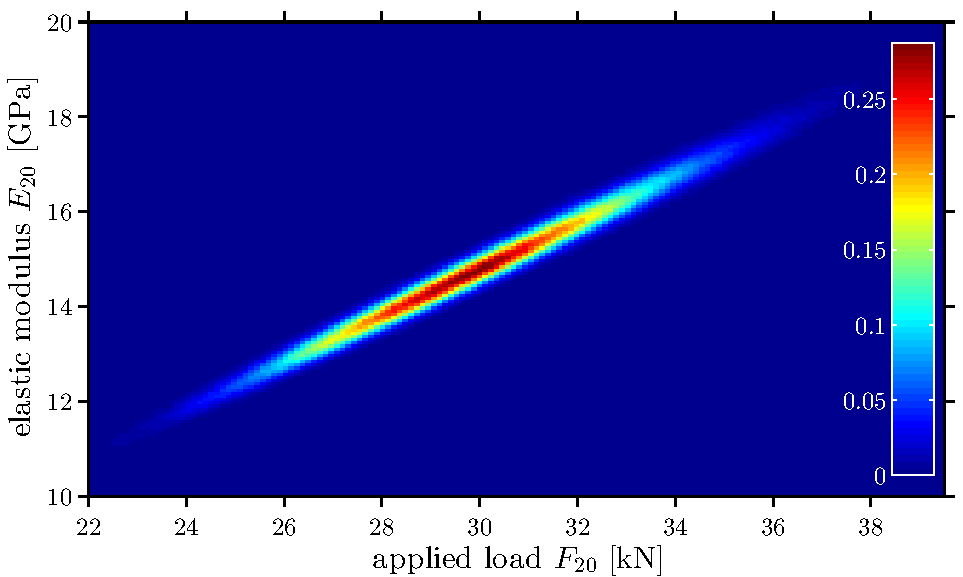
\includegraphics[height=\PEMfigHeight]{fig_PEM_AddPresPost2DLoadParam}
    \caption{2D posterior of \((F_{20},E_{20})\).}
    \label{fig:PEM:AddPres:Post:2DMeanLoad}
  \end{subfigure}%
  \caption[Posteriors of intermediate variables]{Posteriors of intermediate variables.
           In \subref{fig:PEM:AddPres:Post:1DLoad} the posterior marginal of \(F_{23}\) and its structural prior
           \(\mathcal{N}(F_{23} \distparam \mu_{F_{23}},\sigma_{F_{23}}^2)\) with \(\mu_{F_{23}}=\unit[30]{kN}\) and \(\sigma_{F_{23}}=\unit[3]{kN}\) are shown.
           The posterior is centered around the actual value \(F_{23} = \unit[27.24]{kN}\).
           The two-dimensional posterior of \((F_{20},E_{20})\) with \(r_{F_{20},E_{20}} = 0.99\) is shown in \subref{fig:PEM:AddPres:Post:2DMeanLoad}.
          }
  \label{fig:PEM:AddPres:Posteriors}
\end{figure}